En este capitulo se presentan y analizan los resultados experimentales de la
solucion para el problema de al exploracion multirobot coordinada que fue
desarrollada en este proyecto.

% Las pruebas realizadas se dividen sobre tres secciones, en la primera de estas
% se estudia el impacto de construir el GVD de forma incremental. En la segunda
% se comparan las diversas tecnicas de identificacion de objetivos. La tercera
% busca determinar la influencia de las diversas formas de considerar el espacio
% desconocido. 

Las pruebas realizadas se separan en tres secciones segun su proposito. La
primera estudia el impacto de construir el GVD de forma incremental. La segunda
compara las diversas tecnicas de identificacion de objetivos. Y la tercera
analiza la influencia de las diversas formas de considerar el espacio
desconocido. 

% , se presentan los resultados obtenidos y analizan
%  los resultados los cuales son analizados.

% Comentar que estos son cosas generales a todas las pruebas, que en cada una de
% las siguientes secciones se cambian paramtros aislados con el proposito de
% comparar su impacto. (ver capaz que crierios se van a comparar en cada una)

% generales de las pruebas realizadas. Estas 

\section{Especificación de las pruebas}


En lo que resta de esta seccion se especifican las caracteristicas de las
pruebas llavadas a cabo. 

% A lo largo del capitulo se presentan diversas pruebas que buscan comparar ciertos
% aspectos de la solucion desarrollada en este proyecto. En esta seccion se
% especifican las caracteristicas generales que comparten todas las pruebas
% realizadas.


\subsection{Tipos de prueba}
% El proposito de las pruebas presentadas es evaluar el desempeño de diversos aspectos de una
% solucion al problema de la exploción multirobot. 
% Los tipos de prueba quedan definidos 

Las pruebas tienen como proposito validar las variantes presentadas para la
solucion de diviersos aspectos de la del problema de exploracion multirobot.
 
Para lograr esto se definen pruebas consisten en reslover una instancia de
dicho problema, cambiando la forma de resolver cada aspecto a validar.

La instancia del problema de exploracion a resolver es el de explorar un
entorno cerrado con una flota de robots, hasta que no exista espacio sin
explorar.

Debido a esto
las pruebas se dividen en tres secciones, dependiendo del aspecto que se busca comparar.
Dado esto las pruebas

% En la seccion \ref{sec:exp:inc} se compara la construccion incremental del GVD contra
% la no incremental, en la seccion \ref{sec:exp:idobj} se
% comparan los metodos de identificación de objetivos que se describen en la seccion
% \ref{sec:pc:idobj}, finalmente en la seccion 
%  la seccion \ref{sec:exp:desco} analiza la
% influencia de las diversas formas de considerar el espacio desconocido. 

% de objetivos que
% utiliza directamente las fronteras como objetivos, con las que se basan en
% simplicar dichas fronteras, tanto la simplificacion basada en K-Means, como la
% basada en cubrimiento. 

% Dado que se quiere comparar la utilidad entre las variantes para ciertas partes de
% la solución, se definen tipos de prueba según las variantes utilizadas. 

% En esta sección se describe el tipo de prueba que se denominara como $base$. Este consiste
% en una solucion del problema de exploracion multirobot que resuelve la
% identificación de objetivos con el algoritmo de simplificacion de fronteras
% basada en cubrimiento (seccion \ref{subsec:MiSimp}). La construccion de GVD
% incremental como es comentada en \ref{sec:MiConstGVD} con 



\subsection{Metricas}
Las metricas que fueron utilizadas para evaluar el desempeño de la exploracion,
se basan en las que se proponen en \cite{yan2015metrics}.

\subsection{Simulador}
Las pruebas fueron simuladas con Gazebo \cite{gazebo}, el cual fue elegido a
partir del analisis comparativo entre varios simuladores candidatos realizado
en la sección \ref{sec:sim}). 

Debido a que es posible que ejecuciones de un misma simulacion lleven a
distintos resutlados, con el fin de obtener resultados estadísticamente
significativos cada prueba fue ejecutada 20 veces.

\subsection{Hardware}
El simulador junto al resto de procesos necesarios para llevar a cabo una
prueba fueron ejecutados en una computadora personal equipada con un procesador
Intel Core i3-9100F, un procesador gráfico GeForce GTX 660 y 16GB de memoria
RAM.

% Para cumplir con la hipotesis (IV) planteada en \ref{sec:hip}
\subsection{Robot}
Los robots simulados en las pruebas modelan al robot diferencial Pioneer 3-DX
\cite{p3dx}. Cada robot esta equipado con un sensor LiDAR basado en el modelo
URG-04LX-UG01 \cite{hokuyo}, que permite tomar medidas de distancia de hasta
$5.6m$, con una frecuencia de aproximadamente $36hz$. Adicionalente el sensor
fue alterado para tomar medidas en los $360$\textdegree al rededor del robot y
para proporcionar medidas perfectas (sin ruido)\todo{Justificar? Como?}.

\subsection{Flota}

La flota de exploración se compone de cinco robots, ubicados en las posiciones
indicadas en la figura \ref{fig:willow}.%, comenzando por la izquierda. 

Las comunicaciones entre los robots de la flota son sin perdida y de rango
infinito.

\subsection{Entorno}
Las pruebas se realizan en un entrono cerrado que tiene un area explorable de
aproximadamente $10000m^2$. El entorno esta estructurado en habitaciones,
puertas y corredores de varios tamaños. Los unicos obstaculos presentes en él
son paredes y los mismos robots que pueden obstaculizarse entre
sí. Un mapa de este entrono se muestra en la figura
\ref{fig:willow}.

\begin{figure}[H]
  \center
  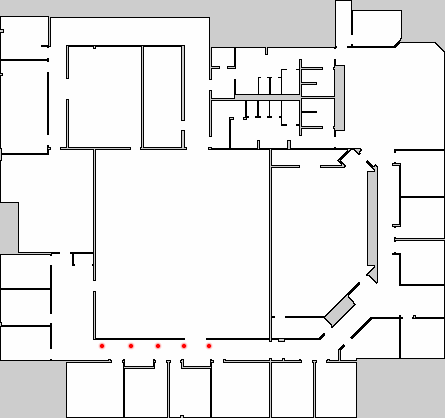
\includegraphics[width=0.5\linewidth]{imagenes/willow/0_250000mRobots2.png}
  \caption[Mapa del entrono utilizado en las pruebas.]{Mapa del entrono utilizado en las pruebas. En negro se indican las paredes, en blanco el espacio libre y en gris el espacio Inaccesible. Las posiciones iniciales de los robots se indican en rojo.}
  \label{fig:willow}
\end{figure} 

El entorno fue construido a partir de un modelo que se encuentra disponible por
defecto en Gazebo, llamado \say{Willow Garage}, el cual se modifico para
reducir el area a exporar y que sea cerrado (sin salidas al exterior).


% \subsection{Tipos de prueba}



% * Pruebas realizadas, cosas generales:
%   * simulador
%   * hardware (de mi pc)
%   * Los robots utilizados
%     * sensor 
%     * robot en si
%   * El entorno de pruebas
%   * Criterios utlizados para analizar los resultados: 
%     * Referencias
%     * Explicar cuales son
%   * Cantidad de pruebas, promedio y varianza

\section{Incrementalidad}\label{sec:exp:inc}

\section{Identificación de objetivos}\label{sec:exp:idobj}

\section{Consideracion del espacio desconocido}\label{sec:exp:desco}

